%!TEX program = xelatex


\documentclass[10pt]{beamer}

\usepackage{ctex}
% \usepackage[colorlinks,linkcolor=red]{hyperref}

\usepackage{graphicx}
\usepackage{float}
% \usepackage[colorlinks, linkedcolor=red]{hyperref}

% for python
\usepackage{listings}
\usepackage{color}

\usepackage{tabularx}
\usepackage{array}

\definecolor{dkgreen}{rgb}{0,0.6,0}
\definecolor{gray}{rgb}{0.5,0.5,0.5}
\definecolor{mauve}{rgb}{0.58,0,0.82}

\lstset{
    frame=tb,
    language=Python,
    aboveskip=3mm,
    belowskip=3mm,
    showstringspaces=false,
    columns=flexible,
    basicstyle={\small\ttfamily},   
    numbers=none,
    numberstyle=\tiny\color{gray},
    keywordstyle=\color{blue},
    commentstyle=\color{dkgreen},
    stringstyle=\color{mauve},
    breaklines=true,
    breakatwhitespace=true,
    tabsize=3,
}



\usetheme[]{Berkeley}

\hypersetup{colorlinks,linkcolor=yellow,urlcolor=yellow}

\mode<presentation>

\title{
    \href{https://github.com/Ls-Dai/Cloud-Sever-Tutorial}{云服务器使用说明和相关规定}
}
\author{联邦学习项目组}
\date{Nov 12, 2020}

\begin{document}
    \maketitle
    \hypersetup{colorlinks,linkcolor=yellow,urlcolor=yellow}

    \section{云服务器概况}
        \begin{frame}
            \frametitle{云服务器概况}
                \framesubtitle{云服务器配置、计费}

                {\small
                \begin{table}[h]
                    \centering
                    \caption{算力对比}
                        \begin{tabular}{|c|c|c|c|}
                            \hline
                            显卡 & 算力(TFLOPS) & 显存(G) & 相对速度 \\
                            \hline
                            Titan XP(A534) & 10.97 & 12 & 1 \\
                            \hline
                            G4 (RTX2080) & 13.45 & 11 & 1.226 \\
                            \hline
                            Tesla T4 & 8.141 & 16 & 0.742 \\
                            \hline
                            Tesla P40 & 11.76 & 24 & 1.072 \\
                            \hline
                            Tesla P100 & 9.526 & 16 & 0.868 \\
                            \hline
                        \end{tabular}
                \end{table}
                }

        \end{frame}

        \hypersetup{colorlinks,linkcolor=yellow,urlcolor=blue}

        \begin{frame}
            \frametitle{云服务器概况}
                \framesubtitle{计费说明}

                {\small
                \begin{table}[h]
                    {\centering
                    \caption{计费说明}
                        \begin{tabular}{|p{0.2\columnwidth}|p{0.6\columnwidth}|}
                            \hline
                            项目 & 单位数量单位时间价格 \\
                            \hline
                            1块RTX2080显卡配上8核i5 CPU & 5.84金币/小时 \\
                            \hline
                            存储空间 & 最低80G,需要 0.02金币/小时。超过80G的部分增加量需为50G的倍数,每增加50G需要 0.015金币/小时,四舍五入保留两位小数 \\
                            \hline
                            传输带宽(按带宽计费) & 5M及以下时为每小时0.03金币/Mbps,多出5M的部分需要增加每小时 0.135金币/Mbps \\
                            \hline
                            传输带宽(按流量计费) & 0.78金币/G,带宽大小可自选,上限100Mpbs \\
                            \hline
                        \end{tabular} \\
                    }
                \end{table}
                {\tiny \qquad \qquad 注:1金币=0.92人民币}
                }

        \end{frame}

    \section{开始使用云主机}
        \begin{frame}
            \frametitle{开始使用云主机}
                \framesubtitle{演示:创建一个适合使用的云主机}

                % \href{https://ai.blsc.cn/#/support/info}{
                %     
\includegraphics{src/img/Tweet.png}
                %     }
                \centering
                \begin{figure}
                    \href{https://ai.blsc.cn/}{
                        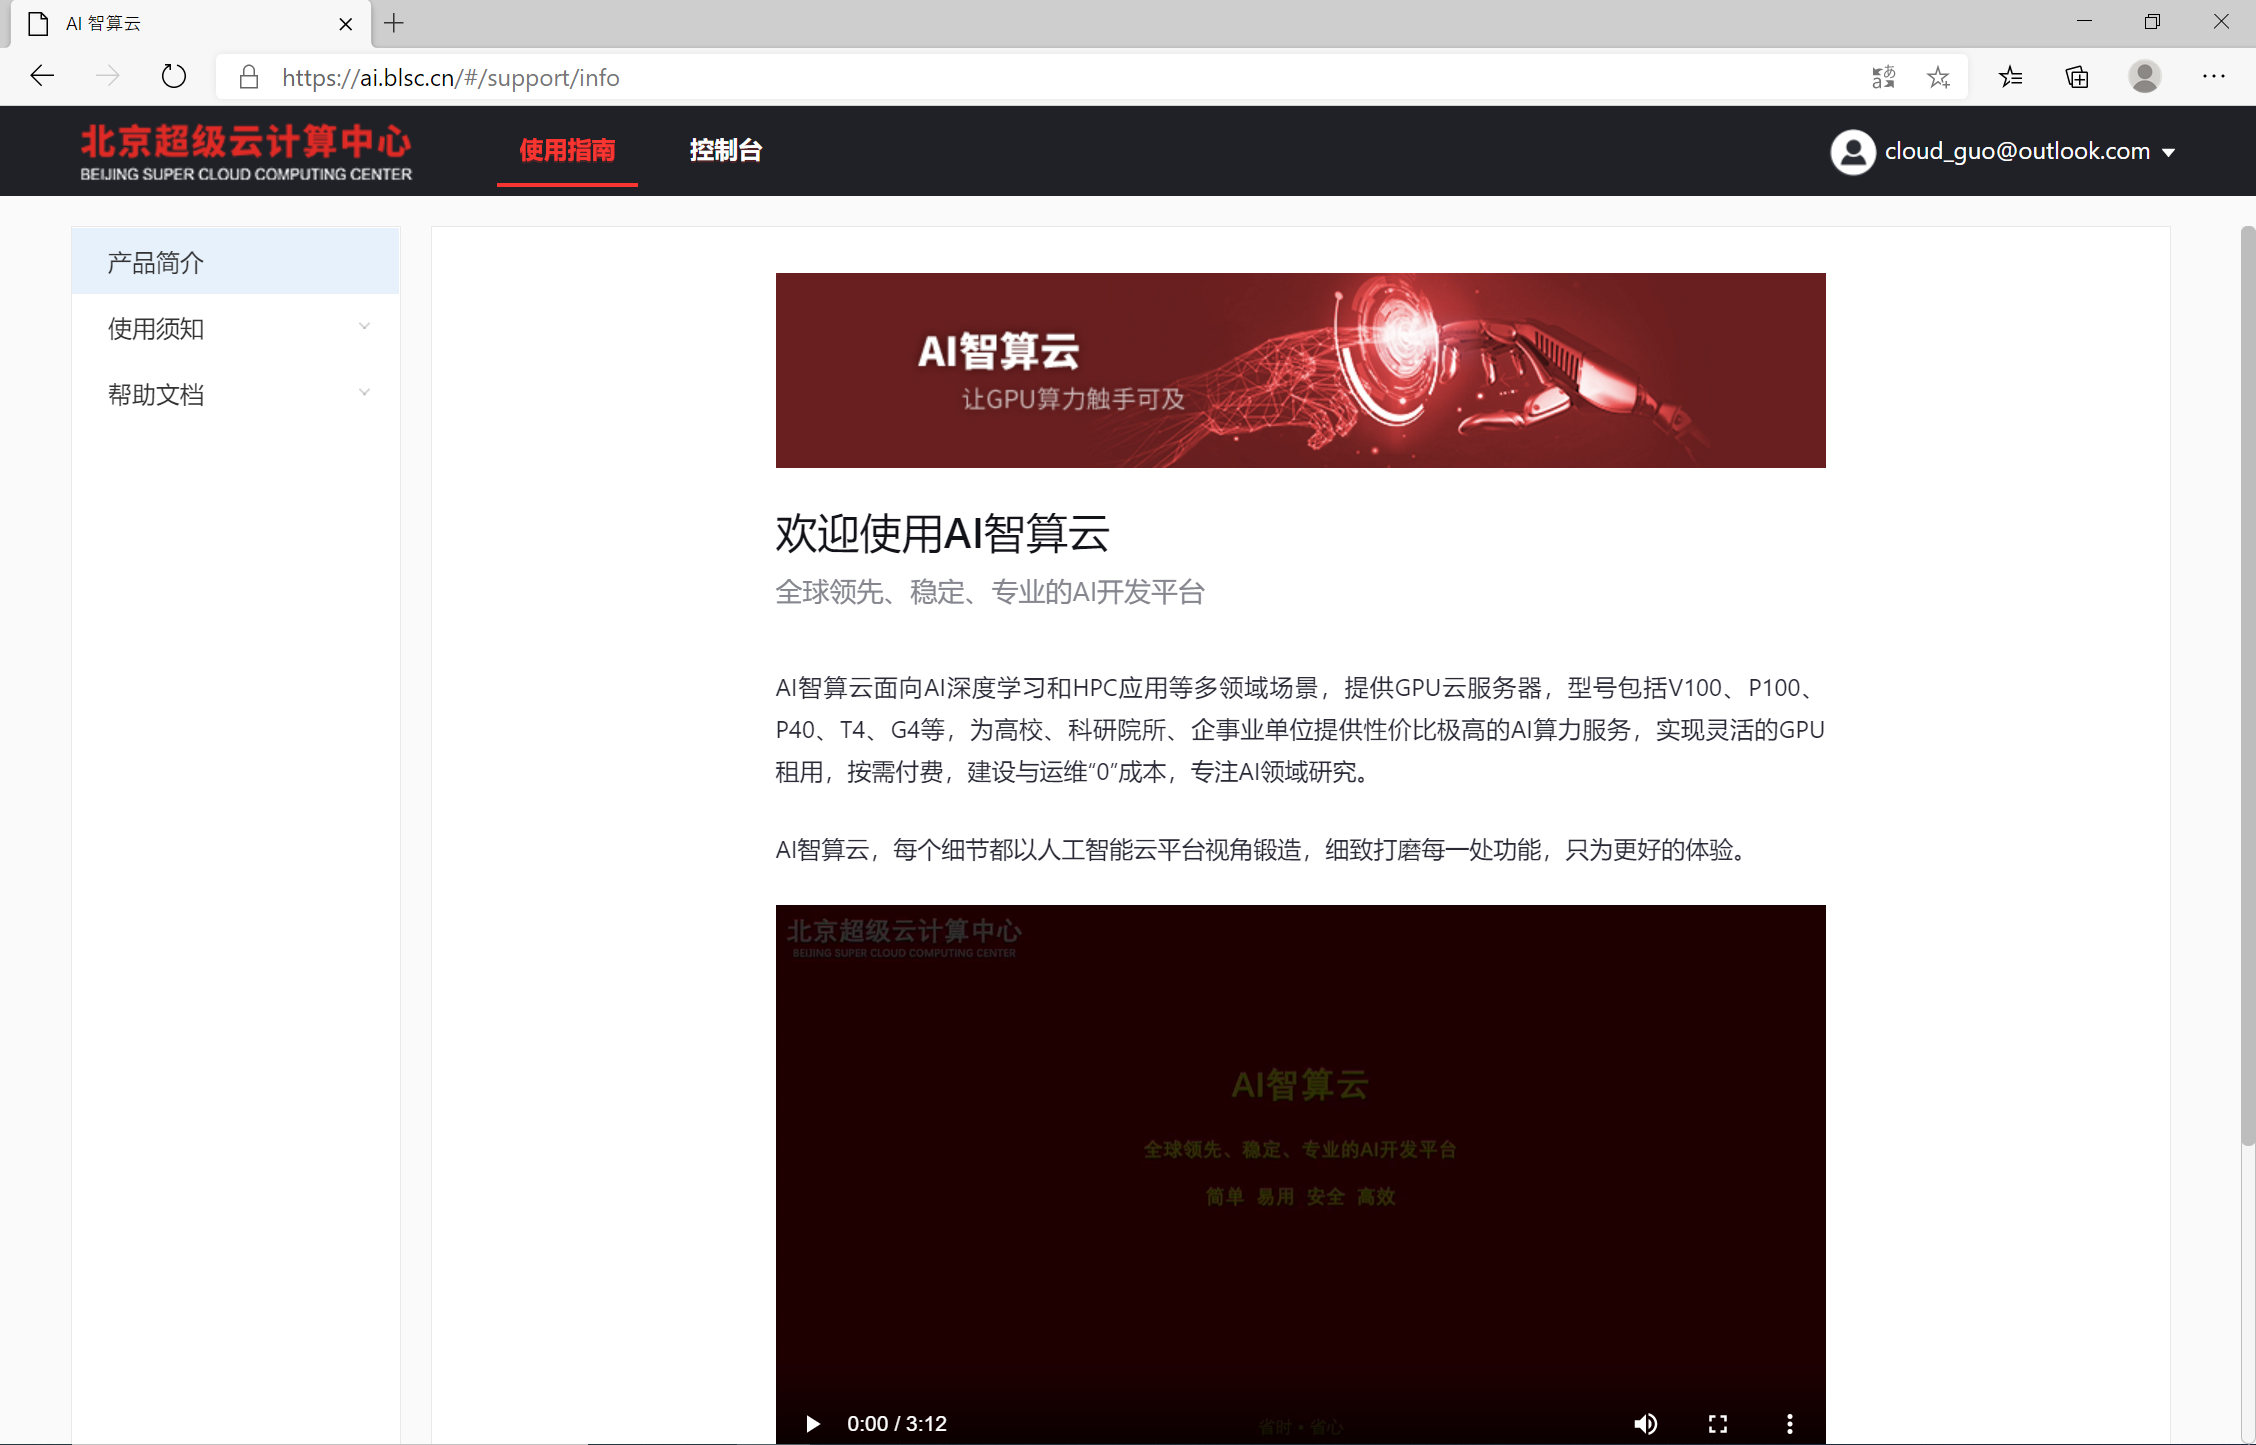
\includegraphics[width=\textwidth]{src/img/Welcome.png}
                        }
                \end{figure}

        \end{frame}

        \begin{frame}
            \frametitle{开始使用云主机}
                \framesubtitle{演示:远程交互}

                % \href{https://ai.blsc.cn/#/support/info}{
                %     
\includegraphics{src/img/Tweet.png}
                %     }
                \centering

                \href{https://mobaxterm.mobatek.net}{
                    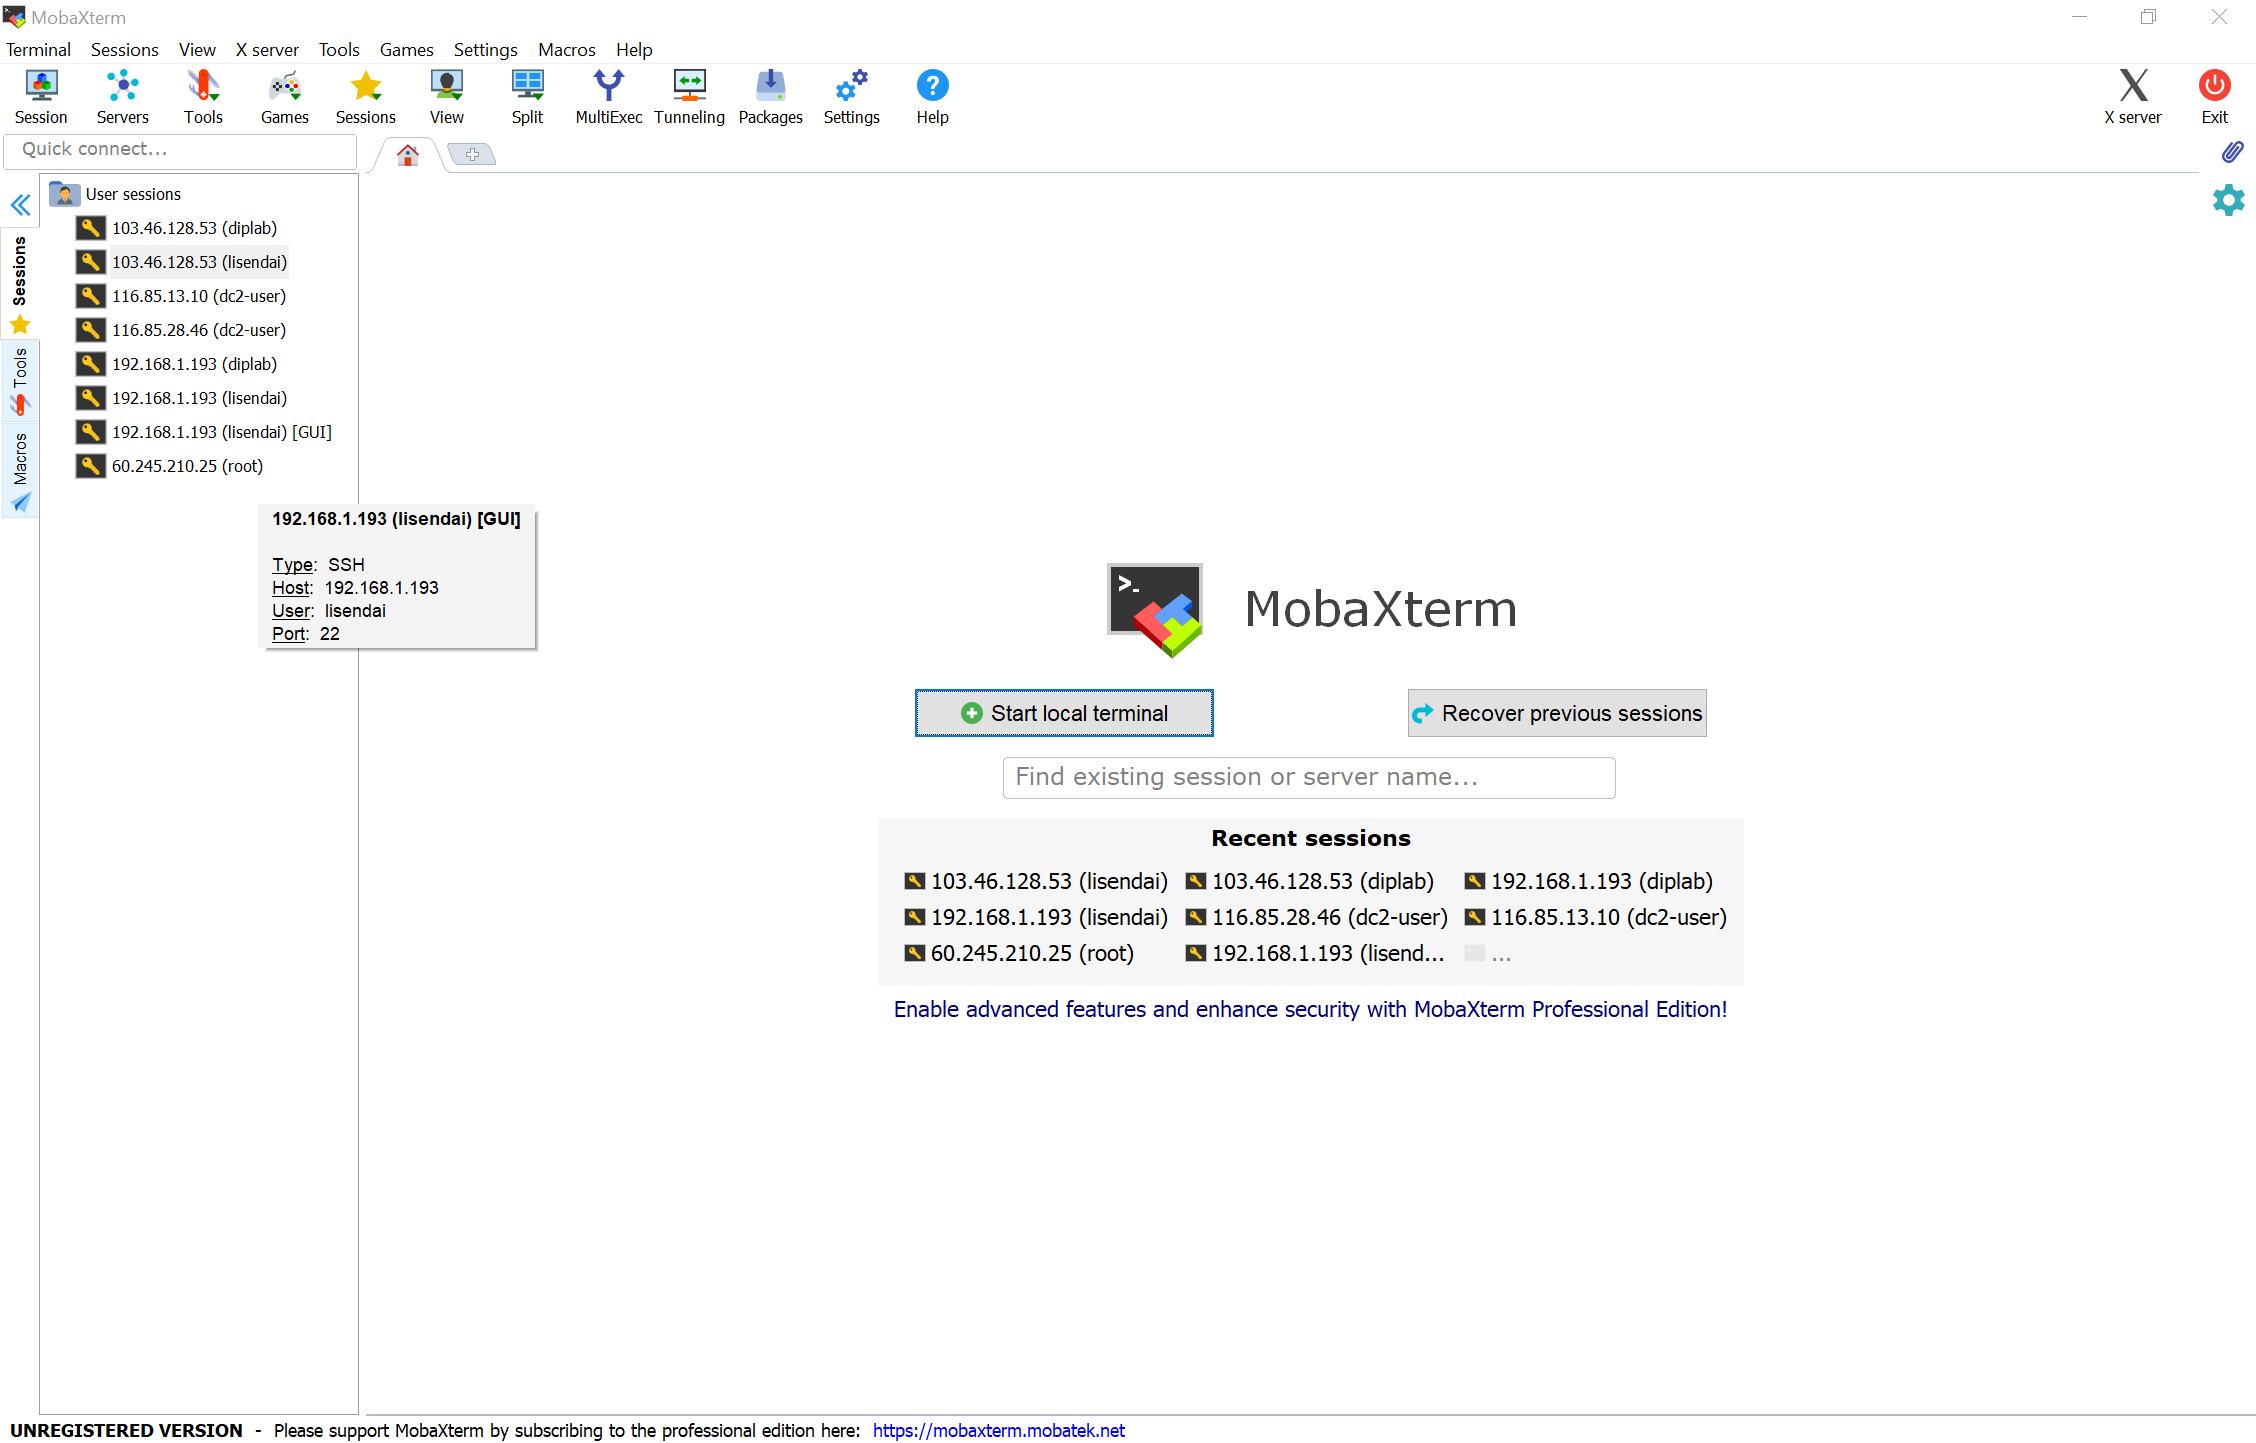
\includegraphics[width=\textwidth]{src/img/MobaXterm.png}
                    }

        \end{frame}

        \begin{frame}
            \frametitle{开始使用云主机}
                \framesubtitle{演示:远程交互}

                % \href{https://ai.blsc.cn/#/support/info}{
                %     
\includegraphics{src/img/Tweet.png}
                %     }
                \centering

                \href{https://mobaxterm.mobatek.net}{
                    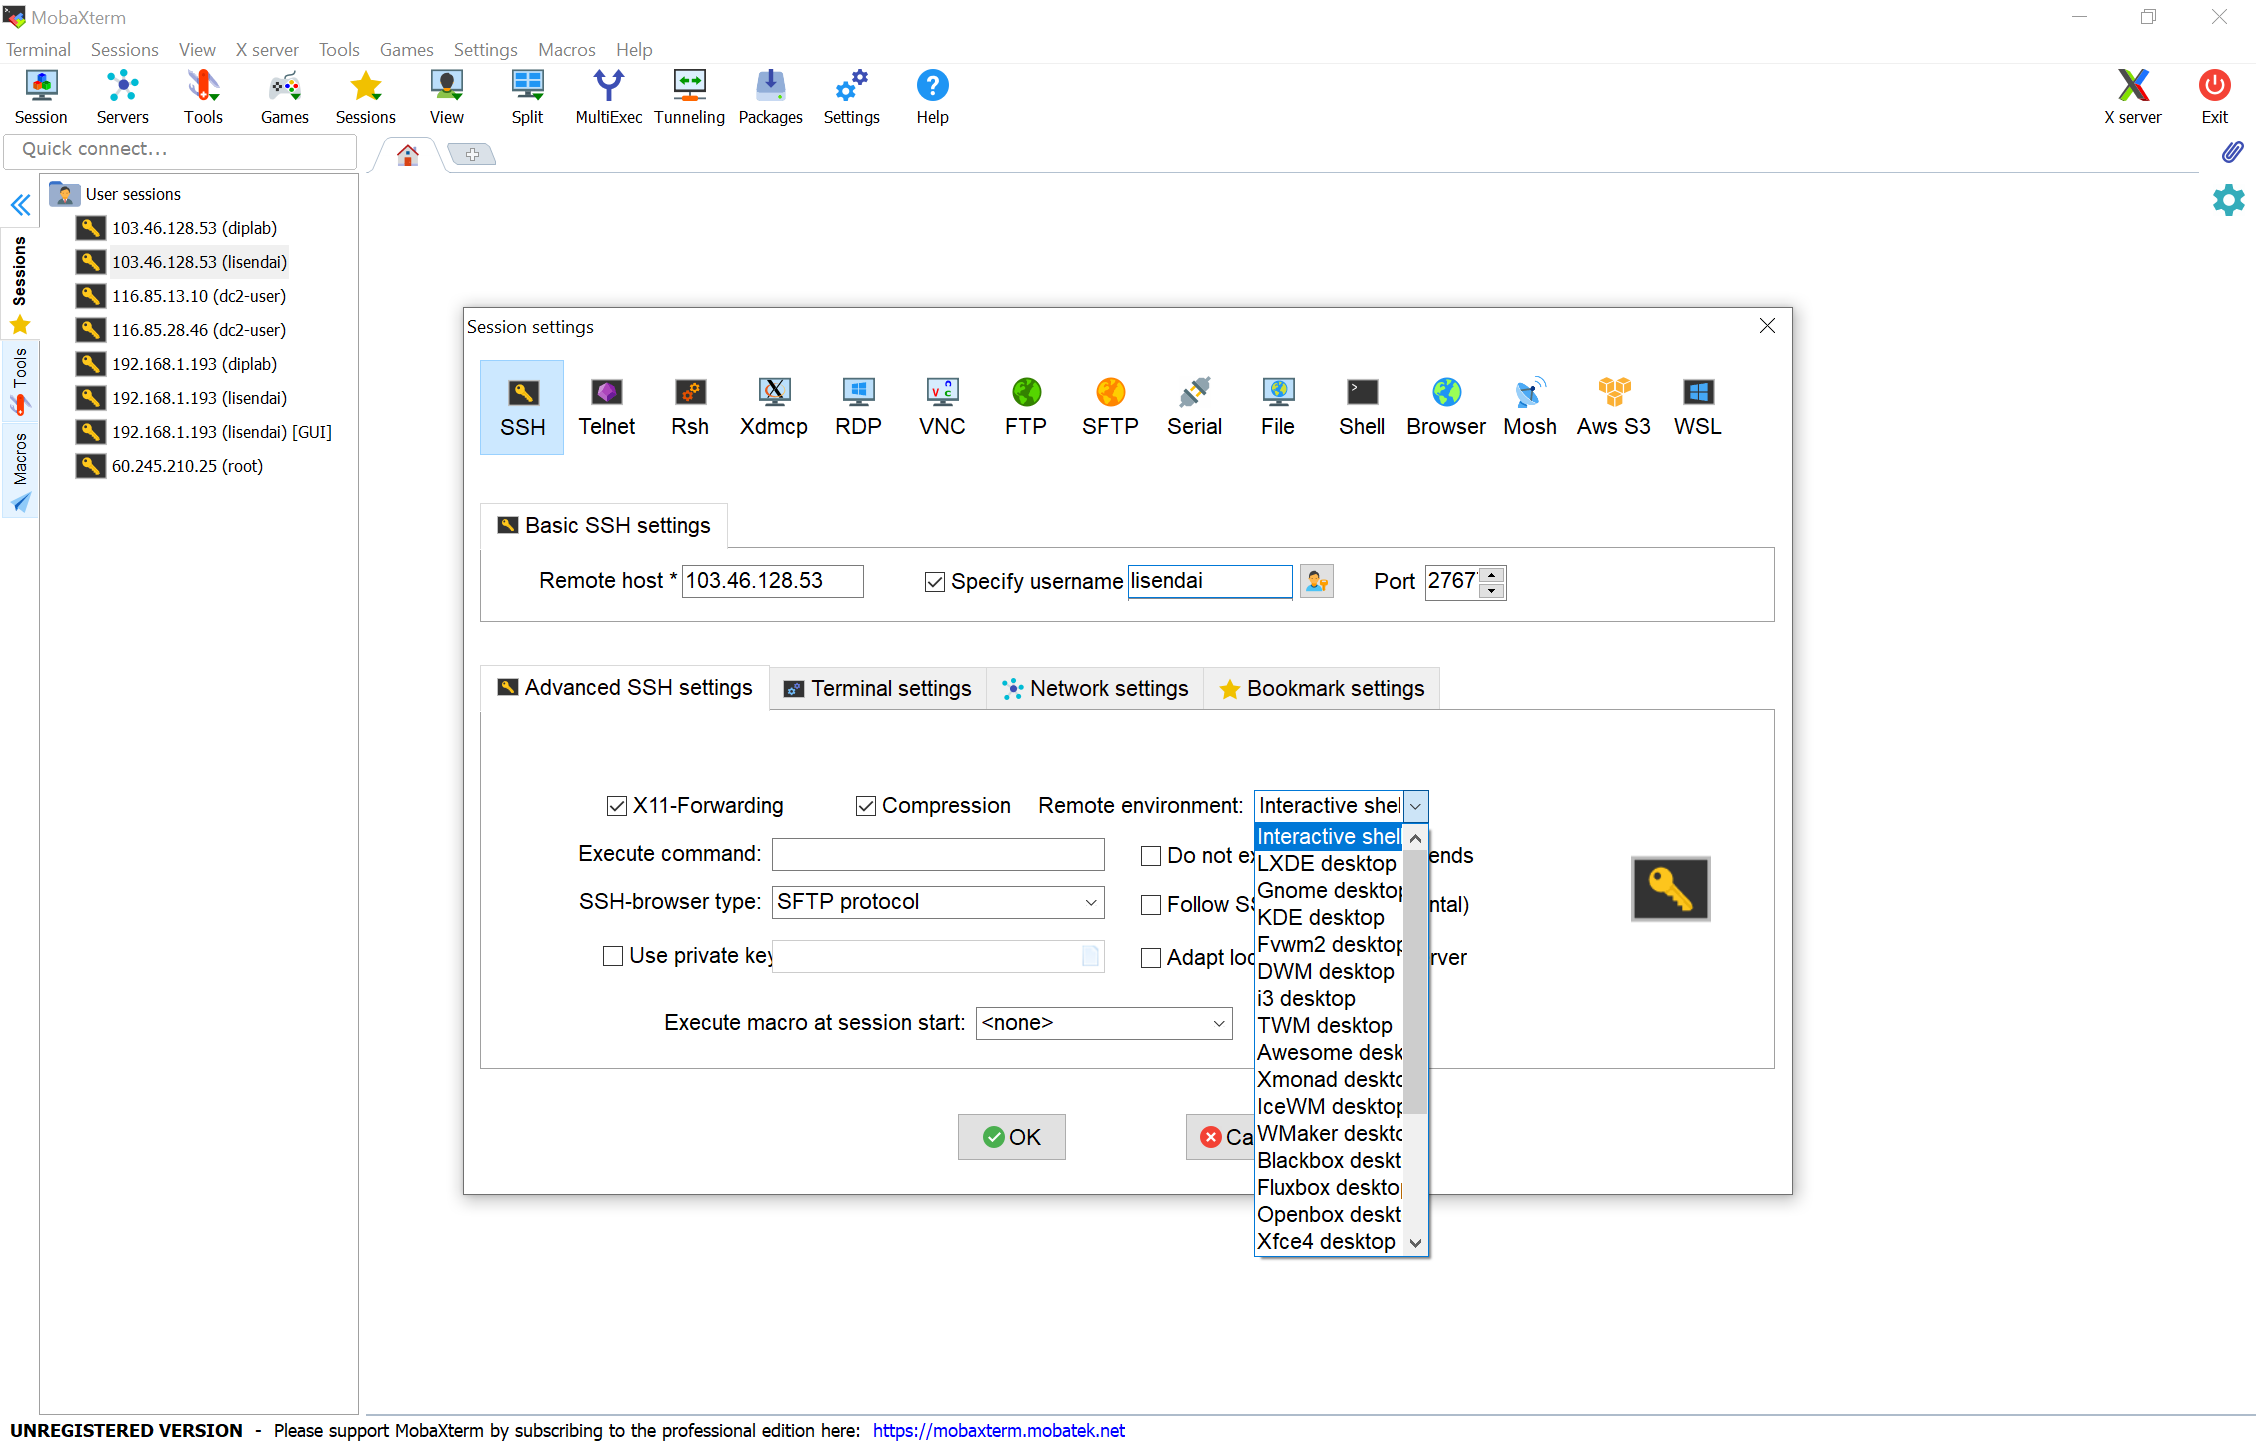
\includegraphics[width=\textwidth]{src/img/Session.png}
                    }

        \end{frame}

        \begin{frame}
            \frametitle{开始使用云主机}
                \framesubtitle{演示:远程交互}

                % \href{https://ai.blsc.cn/#/support/info}{
                %     
\includegraphics{src/img/Tweet.png}
                %     }
                \centering

                \href{https://mobaxterm.mobatek.net}{
                    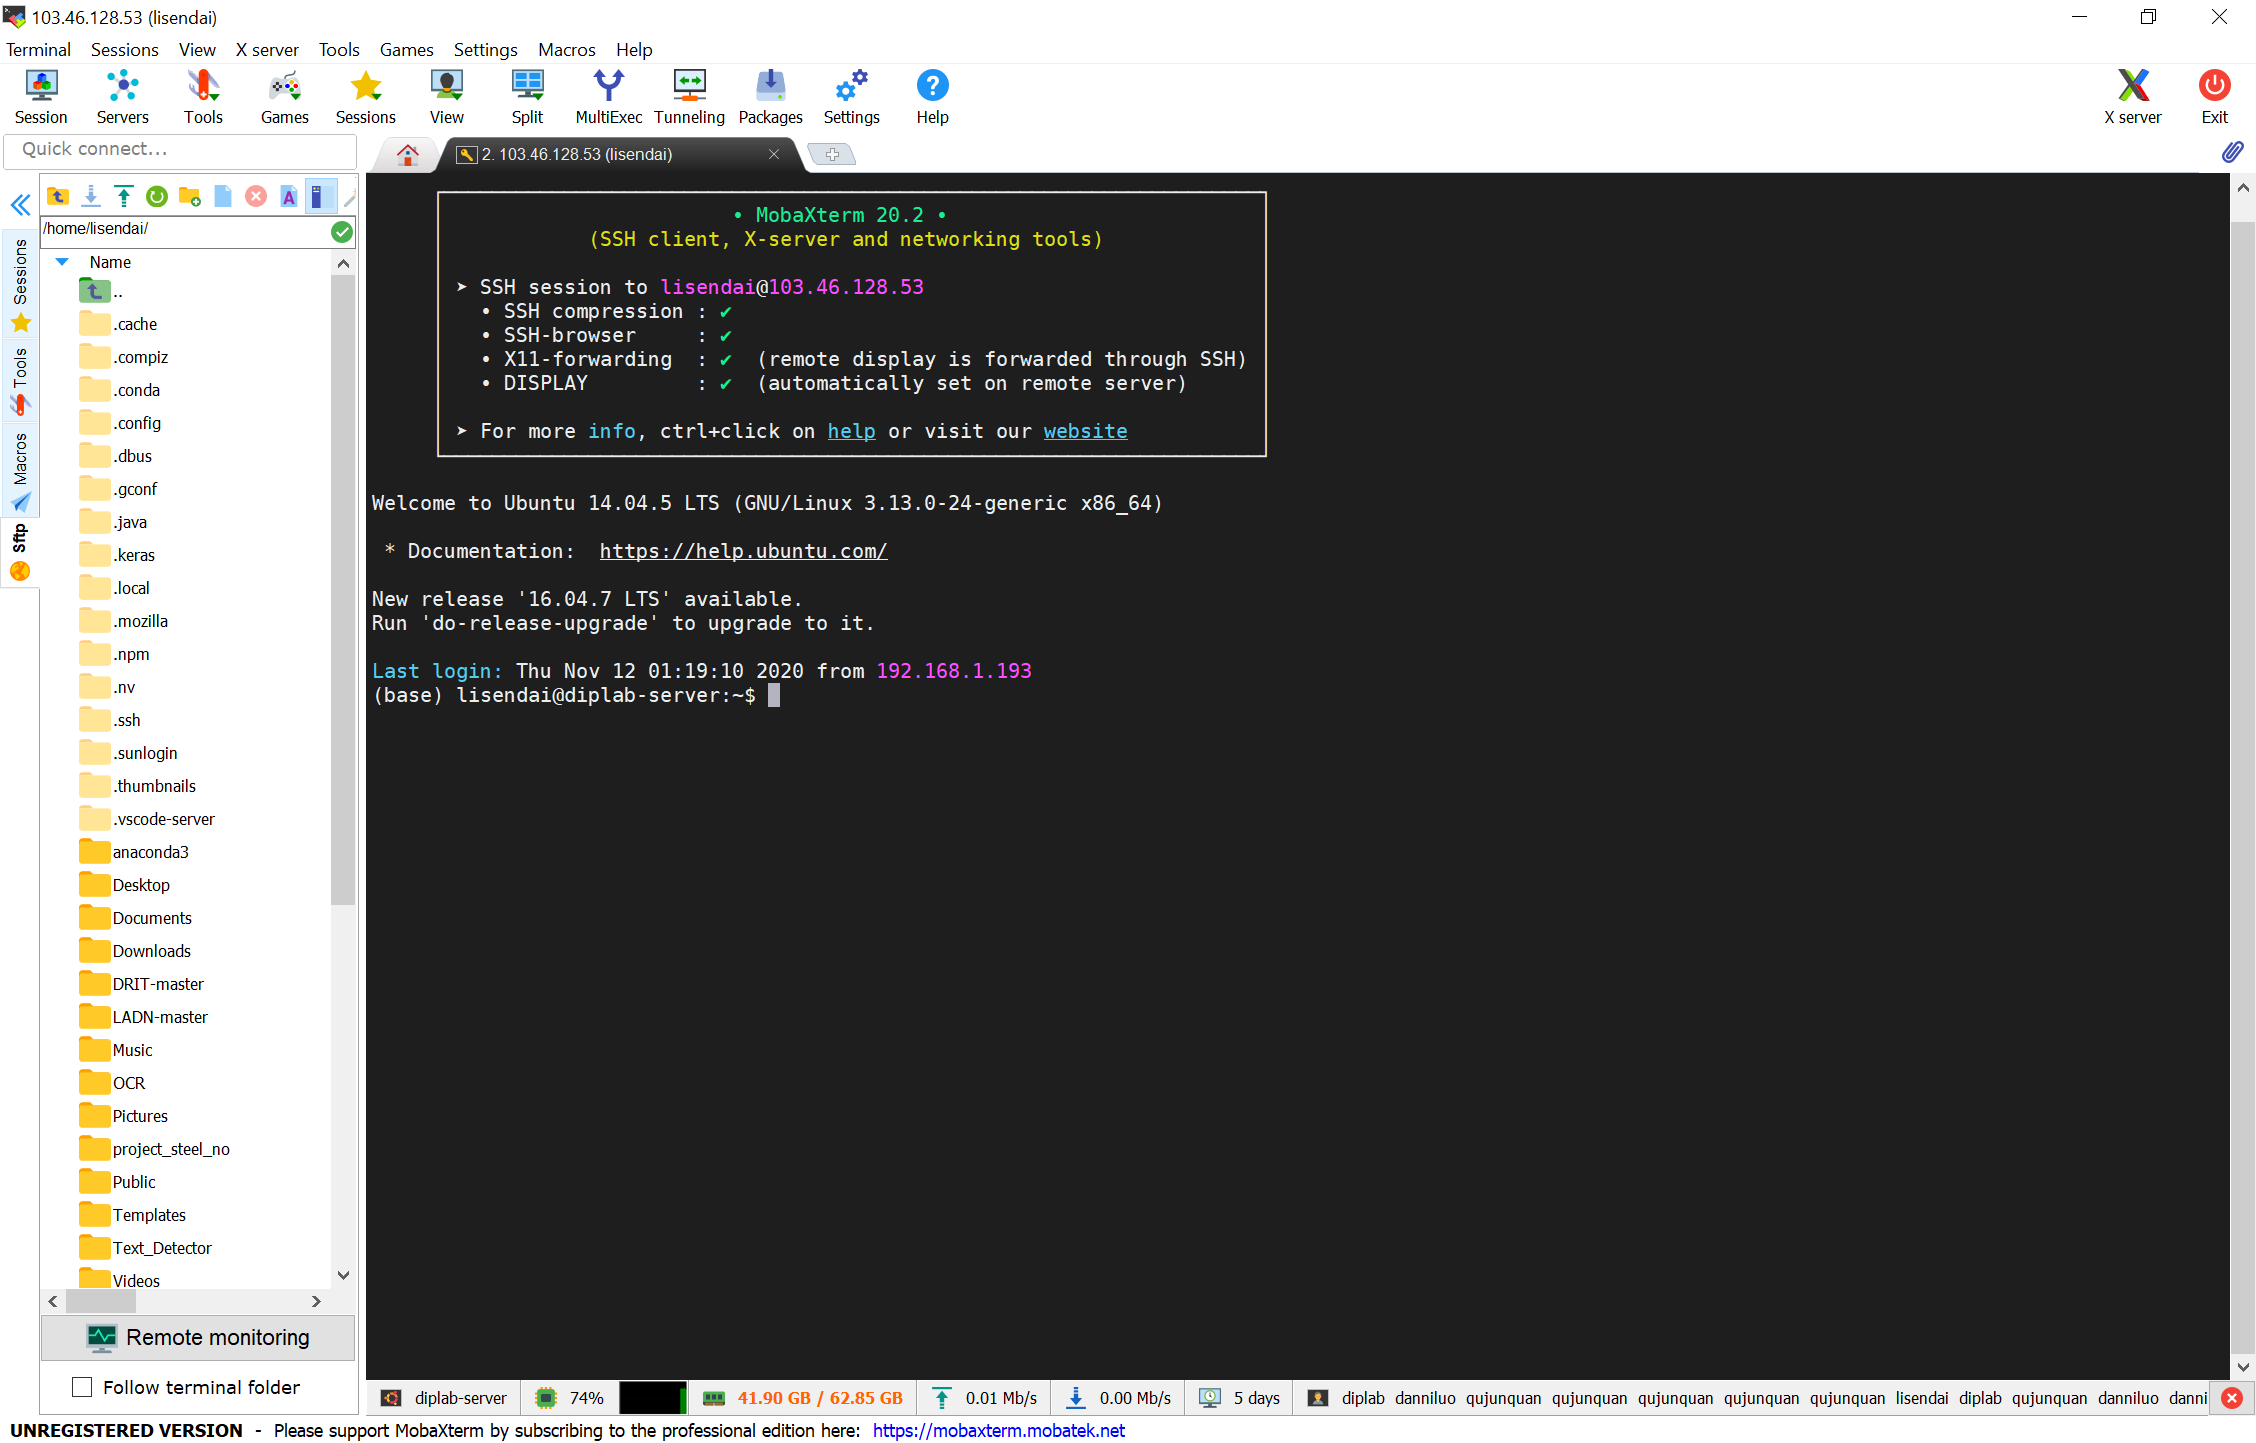
\includegraphics[width=\textwidth]{src/img/SFTP_Shell.png}
                    }

        \end{frame}

    \section{并行计算}
        \begin{frame}[fragile]
            \frametitle{并行计算(PyTorch)}
                \framesubtitle{基本原理}
                    核心代码: \\
                    \begin{lstlisting}
torch.nn.DataParallel                    
                    \end{lstlisting}
                    可将模型发送到多个GPU上进行并行计算,每个GPU都有一个模型的副本。\\
                    训练时,每一批 (batch) 的数据会被均匀地分配到所有GPU上进行处理,计算的梯度会被汇总到原始的模型中进行更新。\\
                    \hspace*{\fill}
                    \begin{itemize}
                        \item 务必保证批的大小(batchsize)大于使用的GPU的数量。
                        \item 在这个训练过程中,因为梯度会被汇总,所以不涉及改变批的大小(batchsize)的问题。
                        \item 因为汇总梯度等原因,GPU(0)一般要被占用更多的显存。
                    \end{itemize}

        \end{frame}

        \begin{frame}[fragile]
            \frametitle{并行计算(PyTorch)}
                \framesubtitle{代码讲解}
                    % Python code
                    \begin{lstlisting}[basicstyle=\small]
import torch.nn as nn
                    \end{lstlisting}
                    \begin{lstlisting}[basicstyle=\small]
gpus = range(num_gpus)
                    \end{lstlisting}
                    \begin{lstlisting}[basicstyle=\small]
torch.cuda.device_count
                    \end{lstlisting}
                    \begin{lstlisting}[basicstyle=\small]
model = nn.DataParallel(model.cuda(), device_ids=gpus, output_device=gpus[0]) 
                    \end{lstlisting}

        \end{frame}

    \section{云服务器使用规则}
        \begin{frame}
            \frametitle{云服务器使用规则}
                \framesubtitle{基本信息管理}
                    账号:\href{mailto: cloud\_guo@outlook.com}{cloud\_guo@outlook.com} \\
                    \hspace*{\fill}
                    \begin{itemize}
                        \item {\href{https://outlook.live.com/owa/}{微软outlook邮箱}}
                        \item {\href{https://ai.blsc.cn/\#/login}{AI智算云}}
                    \end{itemize}

        \end{frame}

        \begin{frame}
            \frametitle{云服务器使用规则}
                \framesubtitle{演示:使用操作流程}
                    \centering

                    \href{https://ai.blsc.cn/\#/cloud/compute}{
                        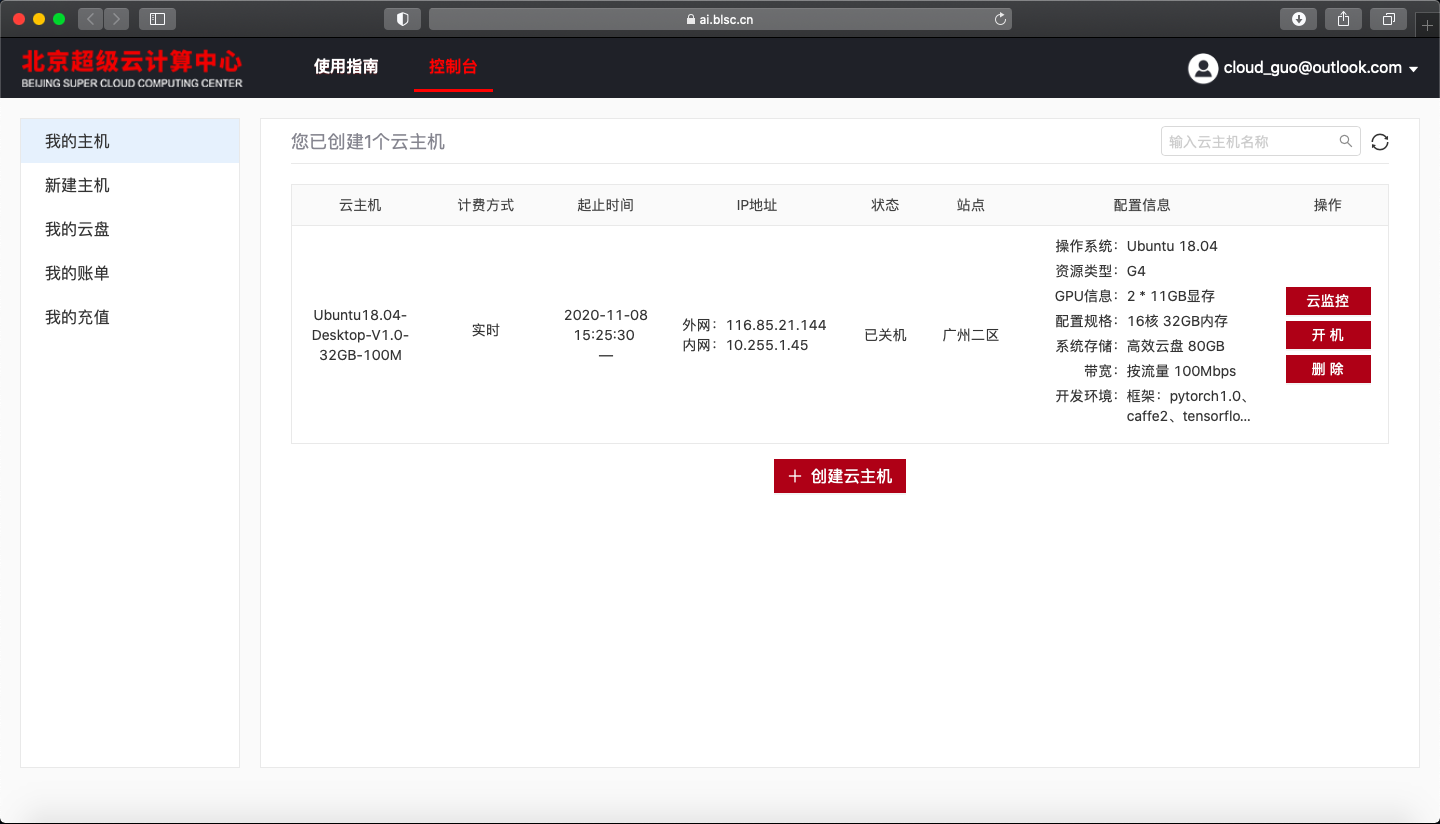
\includegraphics[width=\textwidth]{src/img/Console.png}
                        }

        \end{frame}

        \begin{frame}
            \frametitle{云服务器使用规则}
                \framesubtitle{操作文档}

                {\small
                \begin{table}[h]
                    \centering
                    \caption{操作文档样例}
                        \begin{tabular}{|p{0.04\columnwidth}|p{0.1\columnwidth}|p{0.07\columnwidth}|p{0.12\columnwidth}|p{0.12\columnwidth}|p{0.12\columnwidth}|p{0.12\columnwidth}|}
                            \hline
                            姓名 & IP地址(外网IP) & 开始时间 & 预计结束时间 & 简要的任务说明 & 实际结束时间 & 是否已删除主机 \\
                            \hline
                            &&&&&& \\
                            \hline
                        \end{tabular}
                \end{table}
                }

        \end{frame}

        \begin{frame}[fragile]
            \frametitle{云服务器使用规则}
                \framesubtitle{使用操作流程简述}

                    \lstset{
                        frame=tb,
                        language=bash,
                        aboveskip=3mm,
                        belowskip=3mm,
                        showstringspaces=false,
                        columns=flexible,
                        basicstyle={\small\ttfamily},   
                        numbers=none,
                        numberstyle=\tiny\color{gray},
                        keywordstyle=\color{blue},
                        commentstyle=\color{dkgreen},
                        stringstyle=\color{mauve},
                        breaklines=true,
                        breakatwhitespace=true,
                        tabsize=3,
                    }

                    \begin{itemize}
                        \item [1. ]{
                            确保您的程序已经在A534机器上运行正常,并且已经利用pip或者conda生成环境配置文件。等待在云服务器上使用。\\
                            \begin{lstlisting}
#################### 原机器上 ####################
pip freeze > requirements.txt   # 输出环境版本列表
#################### 新机器上 ####################
# conda create -n env_name    # 创建新的虚拟环境
# source activate env_name    # 激活新建的虚拟环境
pip install -r requirements.txt # 安装环境
                            \end{lstlisting}
                            
                            \begin{lstlisting}
conda env export > environment.yaml # 输出环境版本列表
conda env create -f environment.yaml # 安装环境
                            \end{lstlisting}
                            {\small
                            注:.yaml文件移植过来的环境只是安装了原来环境里用conda install等命令直接安装的包,而利用pip安装的东西没有移植过来,需要重新安装。 \\}
                        }
                    \end{itemize}
        \end{frame}

        \begin{frame}
            \frametitle{云服务器使用规则}
                \framesubtitle{使用操作流程简述}

                    \begin{itemize}
                        \item [2. ]{在操作文档中填写下列信息:姓名,开始时间,预计结束时间,简要的任务说明。}
                        \item [3. ]{通过ip名找到上一次工作的机器,开机,进行运算(或者按需创建新机器)。}
                        \item [4. ]{结束运算,关机,在操作文档中填写下列信息: 实际结束时间。}
                        \item [5. ]{如果此次使用之后,删除主机,在操作文档中填写下列信息: 是否已删除主机。}
                        \item [6. ]{当日安排值班的人于晚上登录账户,按照预计结束时间检查各台机器。关机在预计结束时间之后仍然运行的机器。}
                    \end{itemize}
                    \hspace*{\fill}\\
                    \centering
                    {\large 欢迎大家提出意见。}

        \end{frame}


    \section{相关材料}
        \begin{frame}
            \frametitle{云服务器使用说明和相关规定}
                \framesubtitle{相关阅读材料}
                \begin{itemize}
                    \item \href{https://ai.blsc.cn/\#/support/info}{AI智算云支持} \\
                    \item \href{https://mobaxterm.mobatek.net}{MobaXterm} \\
                    \item \href{https://github.com/Ls-Dai/Cloud-Sever-Tutorial}{云服务器使用说明和相关规定详细文本} \\
                    \item \href{https://www.runoob.com/linux/linux-tutorial.html}{菜鸟Linux教程} \\
                \end{itemize}
                \hspace*{\fill} \\
                \hspace*{\fill} \\
                \hspace*{\fill} \\
                \hspace*{\fill} \\
                \centering
                {\huge 谢谢大家}
        \end{frame}

\end{document}